\begin{figure}
\begin{center}
    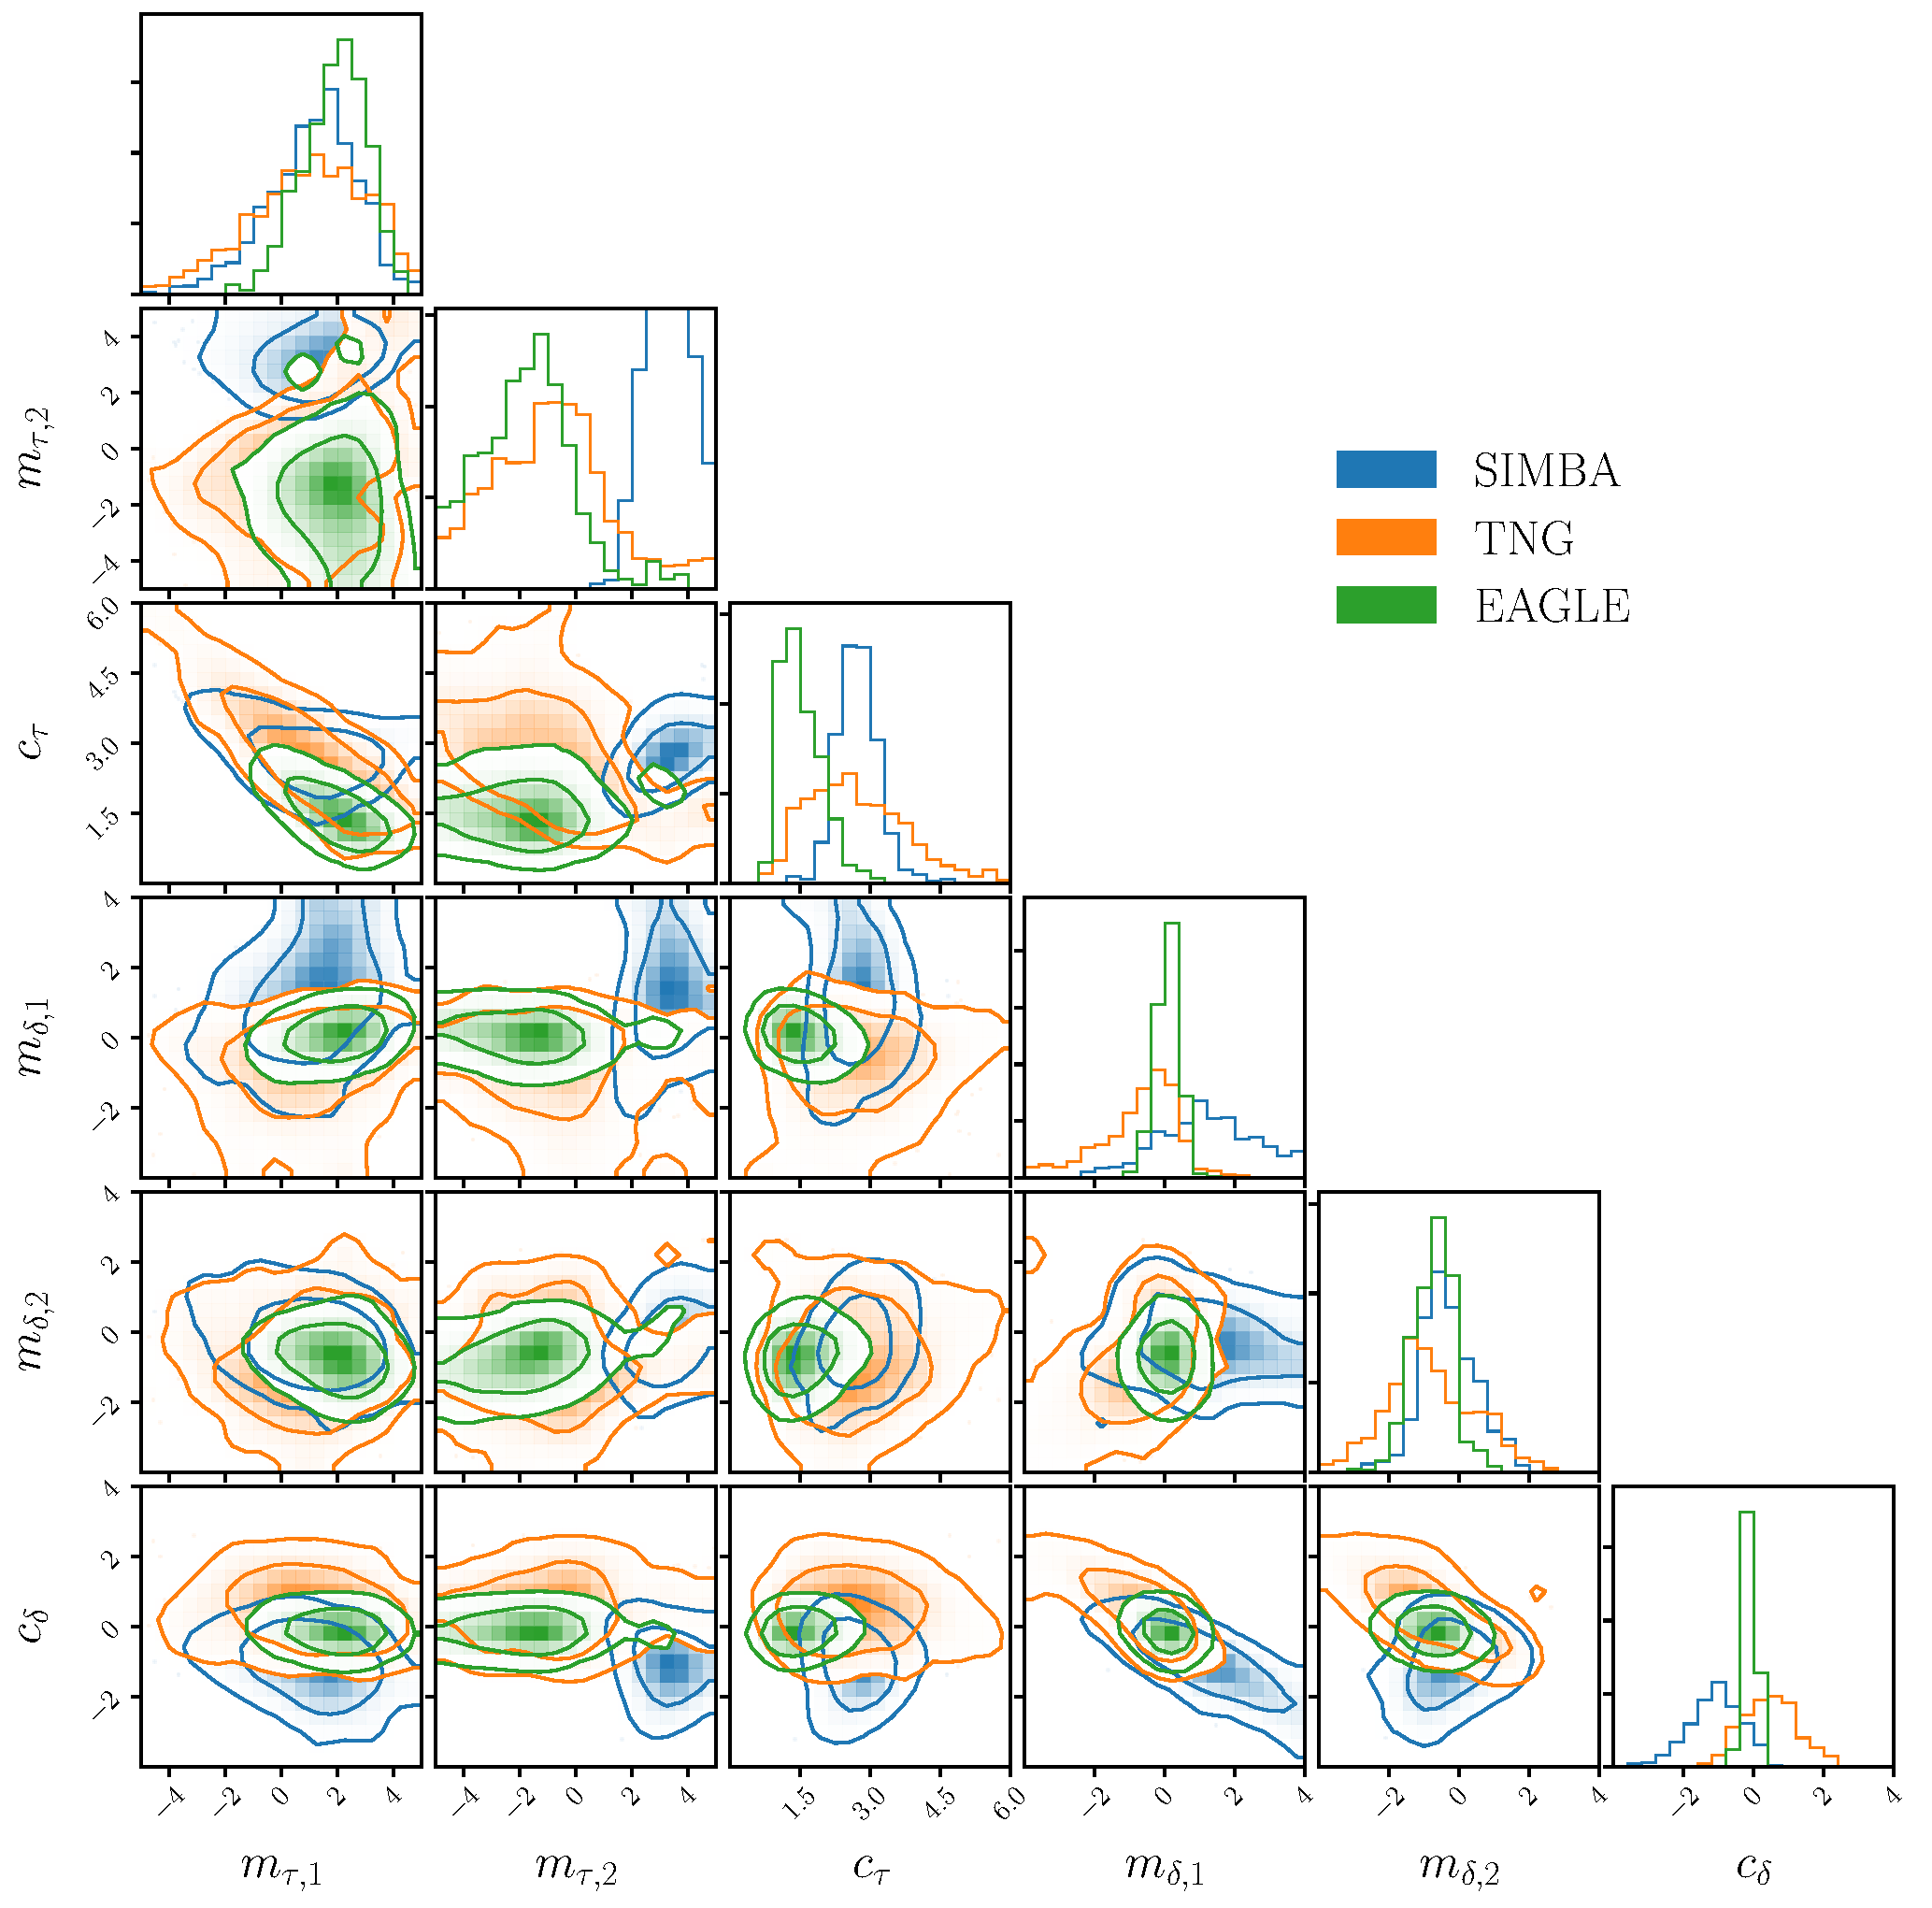
\includegraphics[width=\textwidth]{figs/abc.pdf}
    \caption{\label{fig:abc}
    Posterior distributions of our DEM parameters for the SIMBA (orange), TNG
    (blue), and EAGLE (green) hydro simulations. The contours mark the $68\%$
    and $95\%$ confidence intervals. We describe the parameters in
    Section~\ref{sec:dem} and Table~\ref{tab:free_param} and derive these
    posteriors using Approximate Bayesian Computation (Section~\ref{sec:abc}). 
    In all simulations, dust attenuation increases for higher $M_*$ galaxies 
    ($m_{\tau,M_*} \sim 2$). The simulations also have consistent optical 
    depth amplitudes ($c_\tau$). However, the ${\rm SFR}$ dependence of
    $\tau_V$ is different among the simulations. For TNG and EAGLE,
    star-forming galaxies have lower $\tau_V$; for SIMBA quiescent galaxies
    have lower $\tau_V$. Meanwhile, for the slope offset of the attenuation
    curve, $\delta$, we find little $M_*$ and ${\rm SFR}$ dependence in the
    simulations and that the amplitude ($c_\tau$) is consistent with 0. 
    }
\end{center}
\end{figure}

\begin{figure}
\begin{center}
    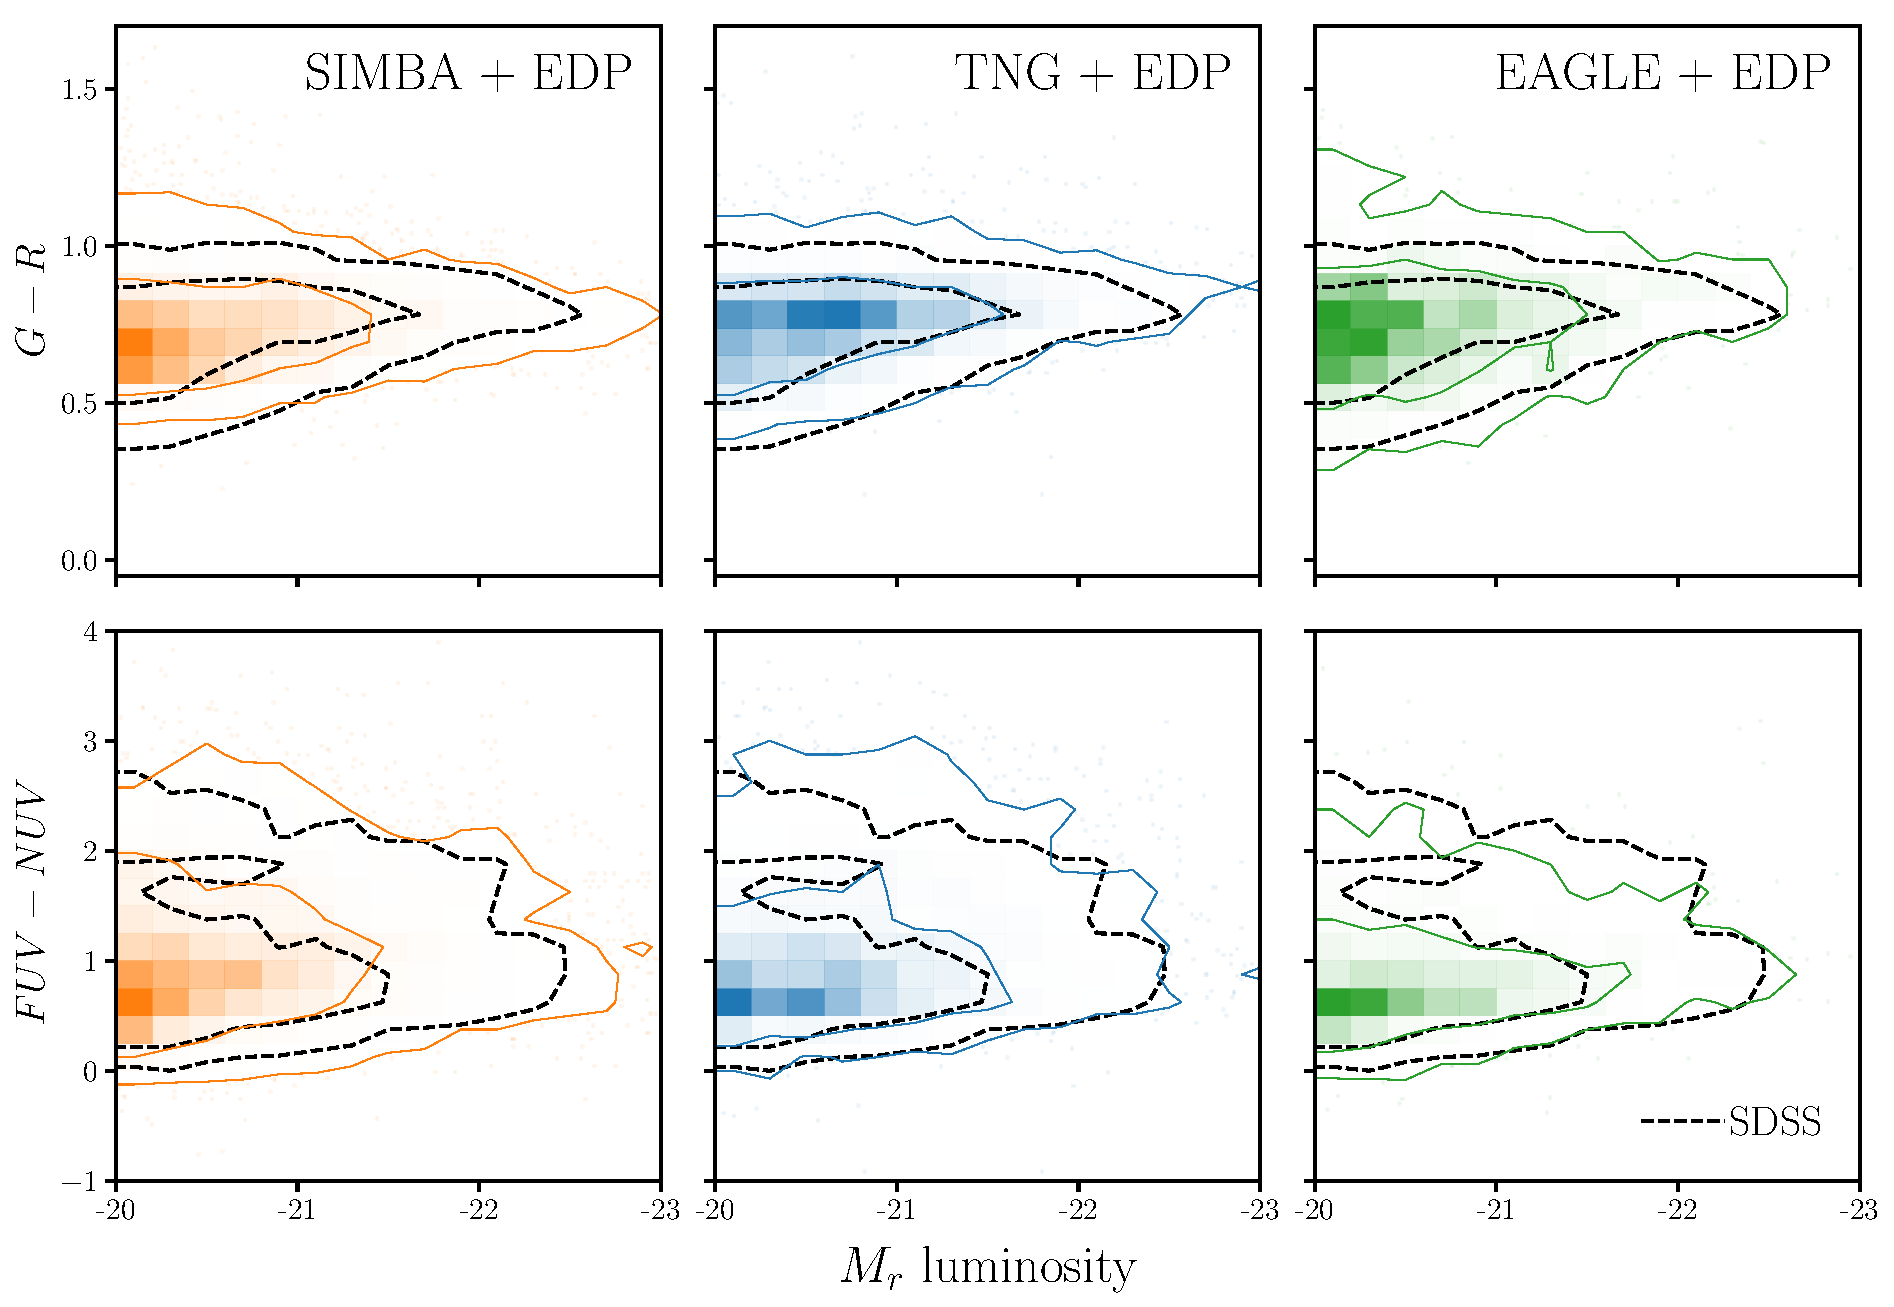
\includegraphics[width=0.9\textwidth]{figs/abc_observables.pdf}
    \caption{\label{fig:dem}
    $(G-R) - M_r$ color-magnitude (top panels) and $(FUV-NUV) - M_r$ (bottom
    panels) relations predicted by the median DEM posteriors for the SIMBA
    (orange), TNG (blue), and EAGLE (green) hydro simulations. For comparison, 
    we include the observables for SDSS in the left-most panel
    (Section~\ref{sec:obs}). The median posterior DEMs produce dramatically 
    different observables than when we do not include any dust prescription
    (Figure~\ref{fig:obs}). Hence, dust must be account for when interpreting 
    and comparing simulations. Moreover, with the DEMs, all three simulations
    produce observables consistent with SDSS. Since different simulations can 
    produce reproduce observations by varying dust, dust significantly limits
    our ability to constrain the physical processes that go into galaxy
    simulations. 
    }
\end{center}
\end{figure}


\begin{figure}
\begin{center}
    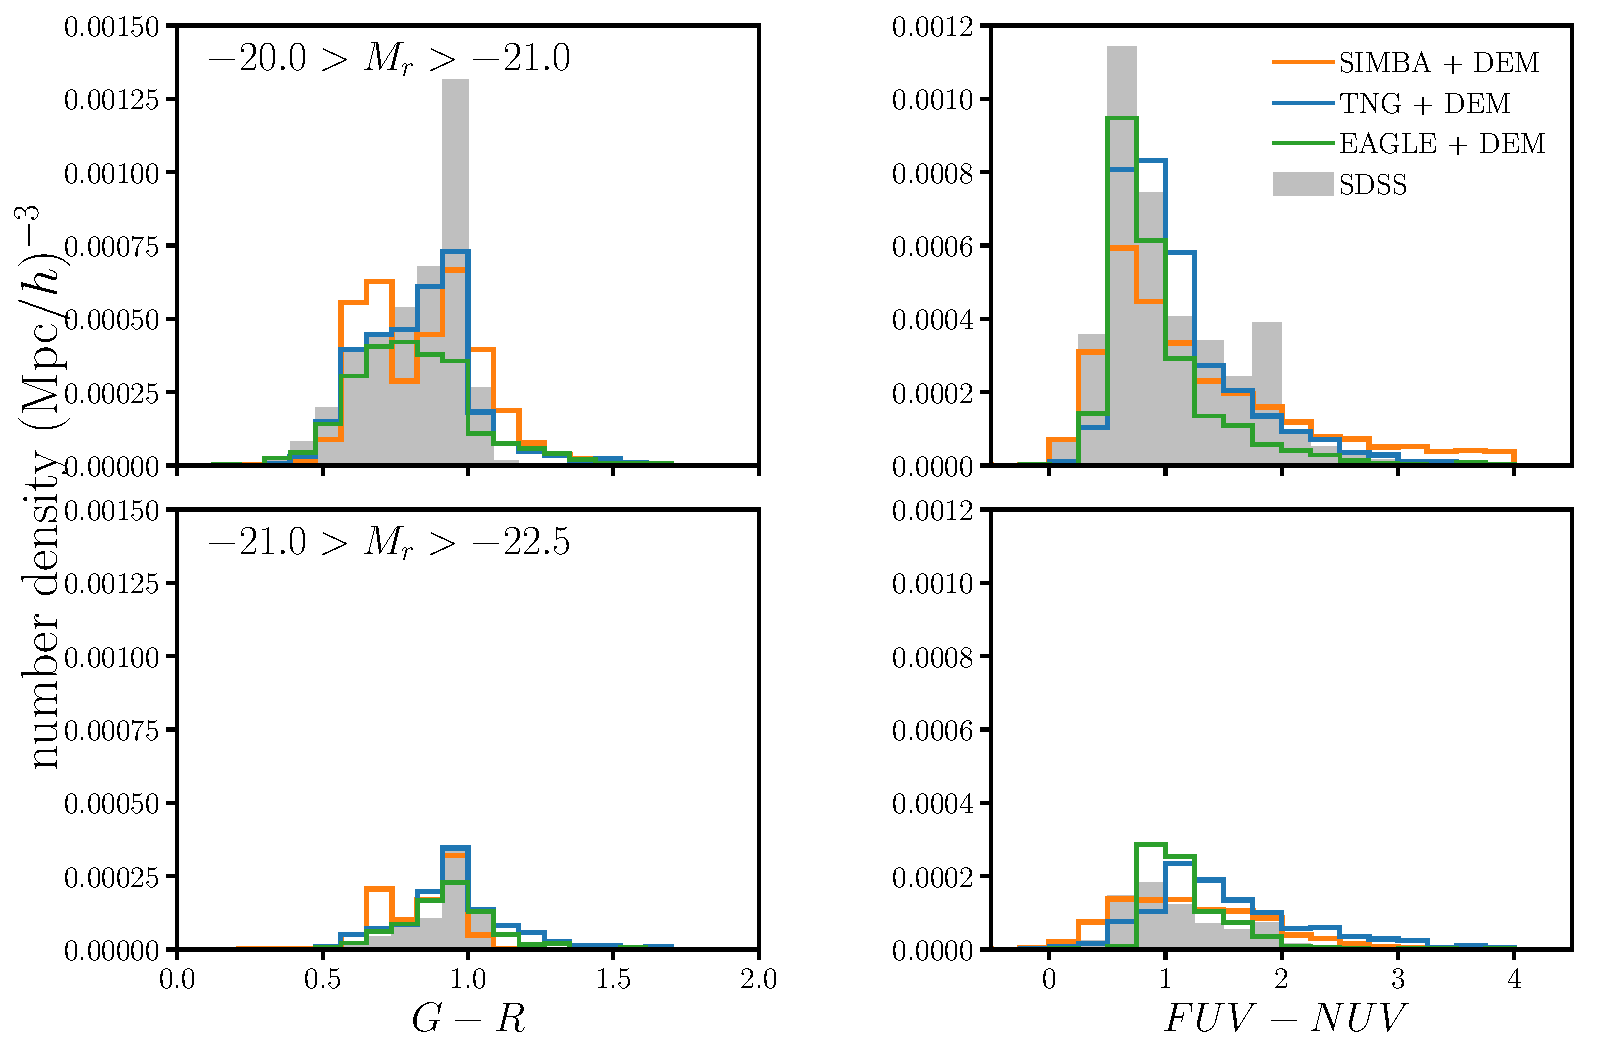
\includegraphics[width=0.85\textwidth]{figs/abc_observables_mr_bin.pdf}
    \caption{\label{fig:demcloseup}
    $G-R$ (left) and $FUV-NUV$ (right) number density distributions for the DEM
    models of the SIMBA (orange), TNG (blue), and EAGLE (green) simulations in
    two $M_r$ bins: $-20 > M_r > -21$ (top panels) and $-21 > M_r > -22.5$
    (bottom panels).  Each of the DEM models are run using the median posterior
    parameter values. In comparison to SDSS (grey shaded), the DEM models predict 
    consistent red sequence and blue cloud positions in the $G-R$ distributions, 
    $FUV-NUV$ peak positions, and number density. {\em Overall the DEM
    models for SIMBA, TNG, and EAGLE produce observables are in good agreement 
    with SDSS.}
    }
\end{center}
\end{figure}


\begin{figure}
\begin{center}
    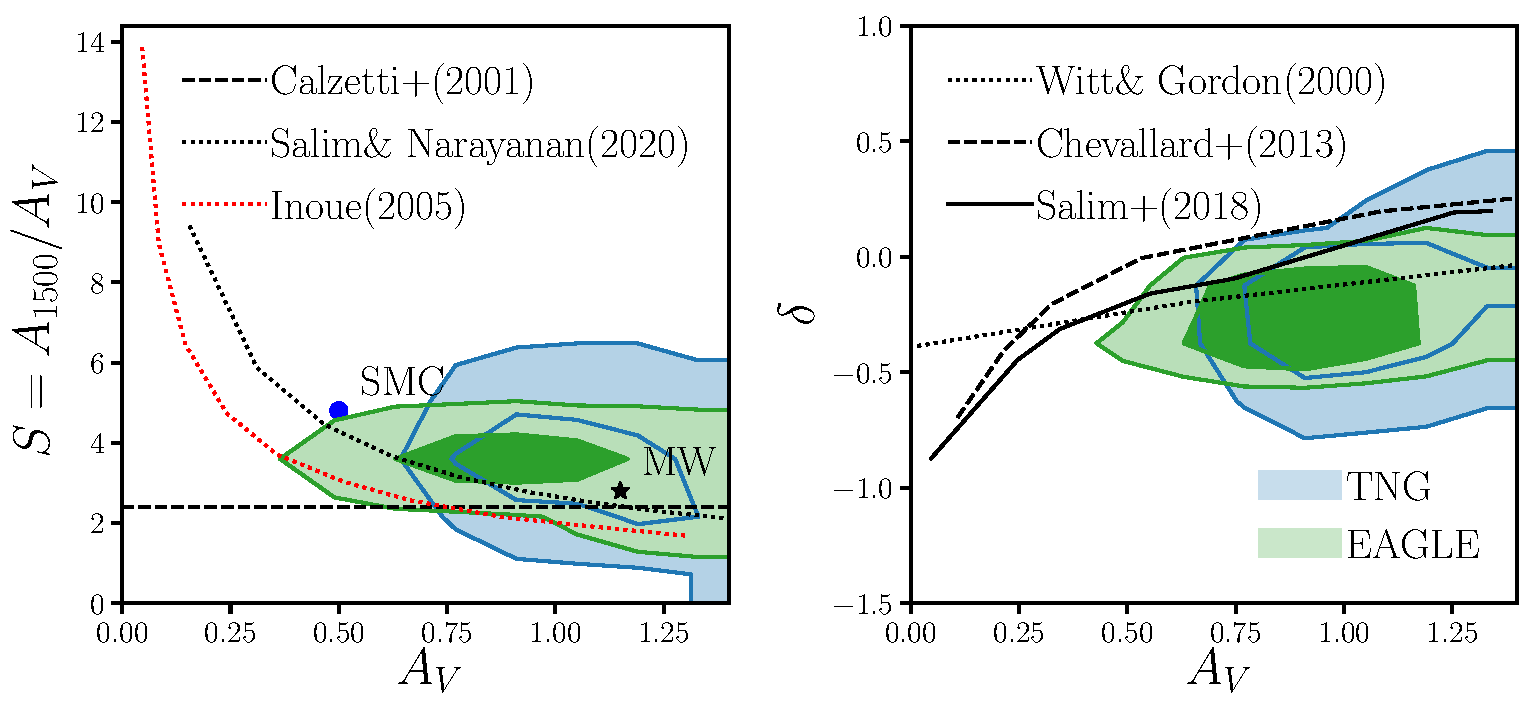
\includegraphics[width=0.85\textwidth]{figs/abc_slope_AV.pdf}
    \caption{\label{fig:slope}
    The attenuation-slope relation for the TNG (bue) and EAGLE (green) DEM
    models. We present the relation usng two different measurements of slope, 
    commonly used in the ltierature: $S = A(1500\AA)/A_V$ (left panel) and
    the slope offset from the \cite{calzetti2001} curve, $\delta$ (right panel).
    The DEM moodels predict an attenuation-slope relation, where the slope is
    steeppr at lower attenuation, consistent with both observations and
    simulation. The DEM models only include masssive galaxies, hence, they do
    not include mnay galaxies with low attenuatiton. At $A_V > 0.5$, however, 
    the DEM models are in good agreement with observations~\cite{salim2020}. In
    fact, the DEM models match the observed attenuation-slope relation 
    better than radiative transfer simulations, which predict attenuation 
    curves that are too shallow~\citep{inoue2005, chevallard2013, trayford2020}
    }
\end{center}
\end{figure}

\begin{figure}
\begin{center}
    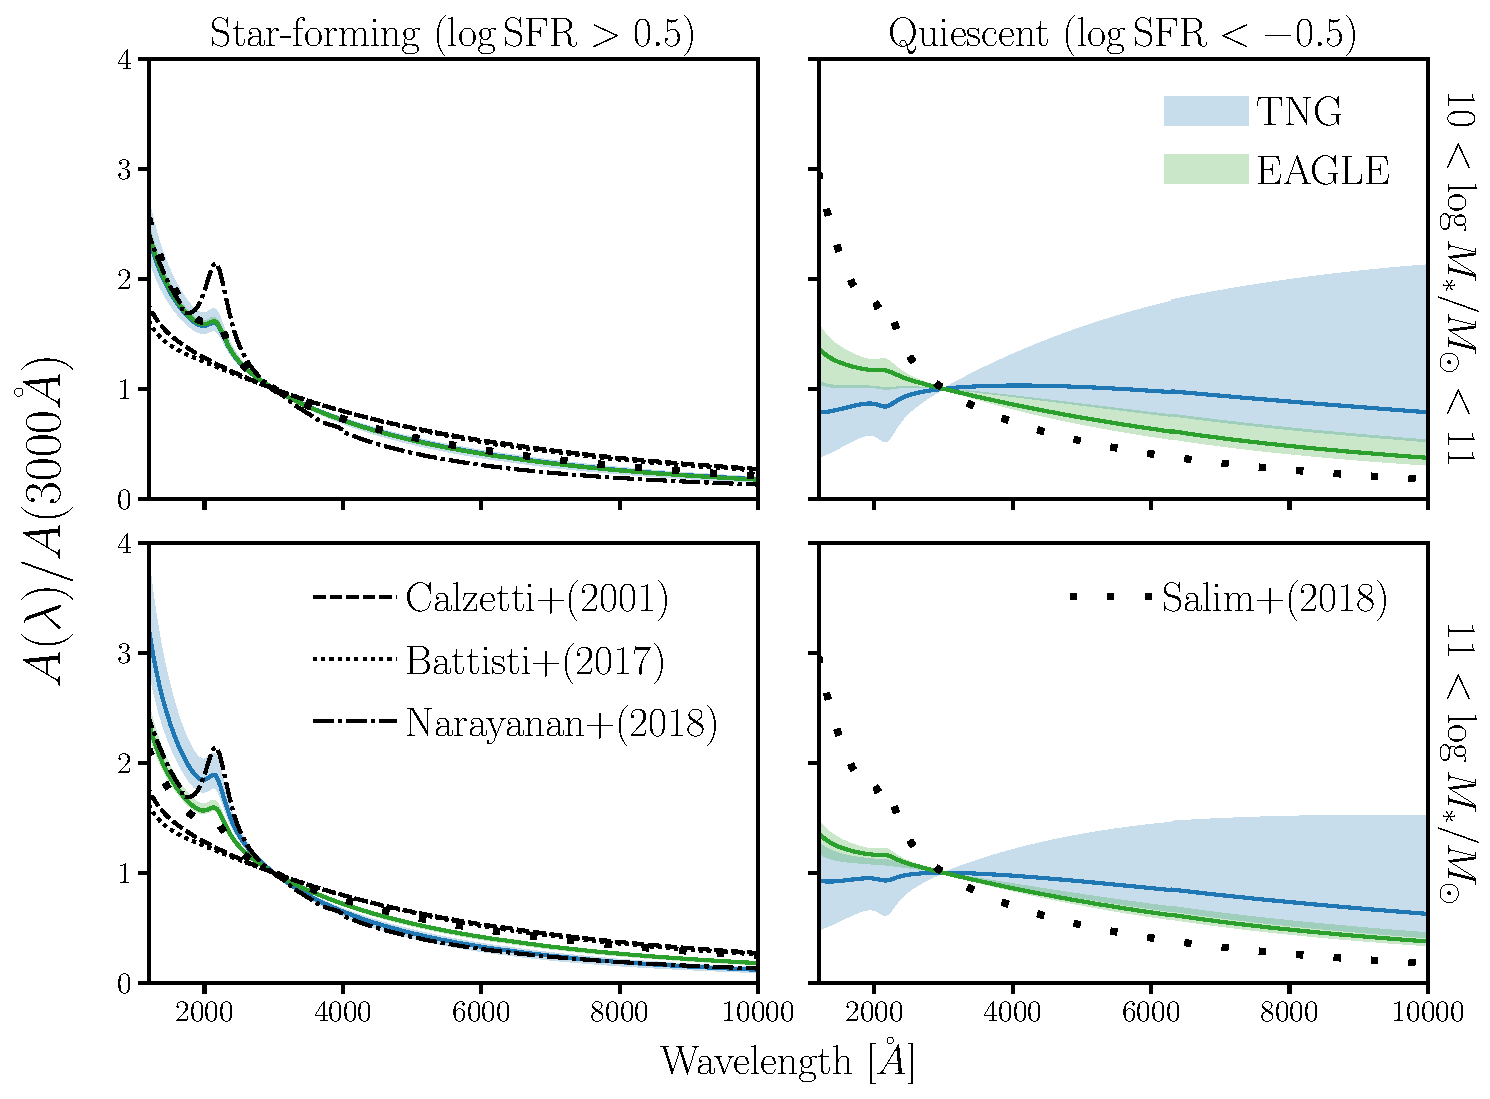
\includegraphics[width=0.85\textwidth]{figs/abc_attenuation.pdf}
    \caption{\label{fig:atten}
    Attenuation curves of the SIMBA (orange), TNG (blue), and EAGLE (green) DEM
    models for low (top) and high $M_*$ (bottom), star-forming (left) and
    quiescent galaxies (right). The attenuation curves are normalized at
    $3000\AA$: $A(\lambda)/A(3000\AA)$. We mark the $1\sigma$ standard
    deviation of the attenuation curves with the shaded region. For comparison,
    we include measurements of $A(\lambda)/A(3000\AA)$ from 
    observations~\citep{caleztti2000, battisti2017, salim2018} as well as
    from simulations~\cite{narayanan2018}. The \cite{calzetti2000} and
    \cite{battisti2017} attenuation curves are shallower than the DEM
    attenuation curves; however, this discrepancy is primarily driven by the
    differences in $M_*$ ranges. For \cite{salim2018}, which probe a similar
    $M_*$ range as our DEM models, we find goood agreement. We also find good agreement with
    median attenuation curve of \cite{narayanan2018} star-forming galaxies. 
    }
\end{center}
\end{figure}

\section{Results} \label{sec:results}
We present the posterior distributions of the DEM parameters for the SIMBA
(orange), TNG (blue), and EAGLE (green) hydro simulations in
Figure~\ref{fig:abc}. The DEM parameters include $\mtaum$, $\mtaus$, and
$\ctau$, which parameterize the $M_*$ dependence, $\sfr$ dependence, and 
amplitude of $\tau_V$, the $V$-band optical depth. $\tau_V$ dictates the
overall strength of the dust attenuation. They also include $\mdeltam$,
$\mdeltas$, and $\cdelta$, which parameterize the $M_*$ dependence, $\sfr$ dependence,
and amplitude of $\delta$, the slope offset of the attenuation curve
(Section~\ref{sec:dem} and Table~\ref{tab:free_param}). The posteriors 
are derived using ABC (Section~\ref{sec:abc}) and the contours mark the 
$68\%$ and $95\%$ confidence intervals. 

In addition, we present the observables predicted by the DEM with median of the
posteriors for the SIMBA (orange), TNG (blue), and EAGLE (green) simulations 
in Figure~\ref{fig:dem}. We include the SDSS observables for comparison
(black dashed; Section~\ref{sec:obs}). The top panels present the $(G-R) - M_r$ 
color-magnitude relations while the bottom panels present the $(FUV-NUV) - M_r$
relations. Without any dust prescriptions, we found that simulations predict
dramatically different observables than SDSS (Figure~\ref{fig:obs}). 
\ch{something about clear bimodality with the red sequence and blue cloud} 
In contrast, {\em using DEMs we produce $(G-R) - M_r$ and $(FUV-NUV) - M_r$
relations consistent with SDSS for all of the simulations}. 

We examine the observables more closely in Figure~\ref{fig:demcloseup}, where
we present the $G-R$ (left) and $FUV-NUV$ (right) distributions in $M_r$ 
bins for the DEM models of the SIMBA (orange), TNG (blue), and EAGLE (green) 
simulations. The top panels contain galaxies with $-20 > M_r > -21$ and the 
bottom panels contain galaxies with $-21 > M_r > -22.5$. In each panel we 
include the SDSS distributions for comparison (grey shaded). These distributions are 
number densities. The positions of the red sequence and blue cloud in the $G-R$
distributions for the DEM models are consistent with the SDSS distribution. 
They also produce $FUV_NUV$ distributions with peaks consistent with
observations. We also find good agreement in the overall normalization
(number density), especially for the $-20 > M_r > -21$ bin. 

There are also a few discrepancies between the DEM models and SDSS observations. 
First, the red sequence in the observed $G-R$ distribution has a sharp red color 
cut-off.  In contrast, we do not find as sharp of a $G-R$ cut off in the DEM models, 
and find a small fraction of galaxies redder than observations. 
Furthermore, while the DEM models for TNG and EAGLE agree with SDSS, the DEM
model for SIMBA overpredicts blue galaxies. \ch{what do we want to do with
SIMBA?} We also find that the TNG and EAGLE DEM models slightly overpredict 
galaxies in the higher luminosity bin and produce a broader $G-R$ distribution.
Nonetheless, Figure~\ref{fig:demcloseup} demonstrates that overall the DEM
models for SIMBA, TNG, and EAGLE produce observables are in good agreement 
with SDSS.

% comparison to literature 
% First EAGLE
Previous works in the literature have also presented models that predict colors
and luminosities for different simulations and dust models and compared them to
observations. For instance, \cite{trayford2015} calculate colors and luminosities 
for $z=0.1$ galaxies using EAGLE with the {\sc GALAXEV} population synthesis models 
and a two-component screen model for dust. Compared to GAMA observations, their
model produces a bluer red sequence and overpredicts luminous blue galaxies~\citep[][Figure
5]{trayford2015}. Although a detailed comparison is difficult since they
compare all galaxies, not just centrals, we note that the DEM models find good
agreement in the positions of the red sequences. Furthermore, for TNG and EAGLE, 
the DEM models do not overpredict blue galaxies. Even for SIMBA, the DEM model
overpredict blue galaxies by a smaller amount.

More recently, \cite{trayford2017} calculated optical colors for the EAGLE simulation using
{\sc SKIRT}, a Monte Carlo radiative transfer code~\citep{camps2015}, to model the dust. 
\cite{trayford2017} compares all galaxies so again, we do not include a direct 
comparison. Compared to GAMA, while they find good agreement with observations 
at intermediate masses, $10^{10.5} < M_* < 10^{10.8} M_\odot$, they again find
a bluer red-sequence at $10^{11.2} < M_* < 10^{11.5}$. While we do not present
comparisons in $M_*$ bins, which compare SED derived $M_*$ to the predicted
$M_*$ from simulations, we find that the position of the red sequence in the
DEM models are in good agreement with SDSS even at $M_* > 10^{11.2}$. Our models, 
however, predict an overall broader color distribution at the high mass end. 
Using the same \cite{trayford2017} EAGLE and {\sc SKIRT} framework,
\cite{baes2019} compared the predicted cosmic spectral energy distributions
(CSED) to observations. While this comparison averages over the galaxy
populations, they find the EAGLE-{\sc SKIRT} CSED overestimates the observed
CSED in the UV regime. Moreover, the $FUV-NUV$ color of their CSED is
significantly higher than GAMA $FUV-NUV$. The DEM models on the other hand, 
predict $FUV-NUV$ in good agreement with observations. 

%\cite{baes2019}: EAGLE+SKIRT SED compparison with GAMA Far UV is not attenuated enough. underrestimates optical and NIR
% then TNG
Besides with EAGLE, \cite{nelson2018} calculated optical colors for the
TNG simulations with a dust model that includes attenuation due to dense gas 
birth clouds surrounding young stellar populations and also attenuation due to 
simulated distribution of neutral gas and metals.
Although they compare the color distribution for all galaxies in bins of $M_*$,
so we cannot directly compare to the DEM models, compared to SDSS they find 
bluer red sequence peak position and narrower blue cloud. We find neither of
these discrepancies between the DEM models and SDSS. 
\ch{restatement of how the DEM models have the flexibility to reproduce the
optical and UV color-magnitude relationship.}

The simulations with DEMs predict observables in agreement with observations 
despite the significant differents in the SMFs and $M_*$-SFR relations 
(Figure~\ref{fig:smf_m_sfr}). In other words, the DEM has the 
flexiblity to reproduce observations even when simulations predict galaxy
populations with significantly different physical properties. We emphasize that
the DEM is based on the standard prescriptions for dust attenuation and, thus,
serve as a flexible parameterization within the bounds of our current
understanding of dust in galaxies.

Figures~\ref{fig:dem} and~\ref{fig:demcloseup} highlights two key points. First, any comparison of
simulations must account for dust. Dust entirely changes the predictions of
simulations in observables-space. Without dust, we did not find bimodality in
the color-magnitude relation.
Fortunately, the DEM provides a simple framework
for including dust motivated by attenuation laws and correlations with the
physical properties of galaxies. 
Second, the current limiations in our understanding of dust in galaxies 
significant impedes our ability to understand galaxy formation from simulations. 
To robustly interpret any comparison of simulations, we would need to
marginalize over dust (\emph{e.g.} DEM parameters). Since DEMs can produce
consistent observables for a range of simulations, marginalizing over dust
would leave little constraining power on the subgrid prescriptions (\emph{i.e.}
galaxy physics) of the simulations. 

% what we learn about AV - galaxy property connection  
The DEMs demonstrate that simulations can closely match observations by varying
dust attenuation. They therefore illustrate how dust is a major bottleneck for
directly interpreting galaxy simulations for insights into galaxy formation. In
addition, DEMs also provide some insight into dust. Given our parameterization
(Section~\ref{sec:dem}), it is especially easy to interpret correlation between
dust attenuation and galaxy physical properties. For instance, the posteriors of
DEM parameters in Figure~\ref{fig:abc} reveal a
number of consistent trends across the simulations. In all three simulations, we find significant positive
$M_*$ dependence of $\tau_V$: $\mtaum \sim 2$. Regardless of the underlying
hydro simulations, we find that {\em galaxies with higher $M_*$ have overall higher 
dust attenuation}.

This $M_*$ dependence is consistent with prevoius works in the literature.
The seminal work of \cite{burgarella2005}, for instance, found significant
positive $M_*$ dependence in $FUV$ attenuation in NUV-selected and FIR-selected
samples of \cite{buat2005} and \cite{iglesias-paramo2006}. \cite{garn2010} also
find positive $M_*$ dependence in Balmer decrement-based H$\alpha$ attenuation
in ${\sim}90,000$ SDSS star-forming galaxies. \cite{battisti2016} similarly
find higher Balmer optical depth for higher $M_*$ in ${\sim}10,000$
star-forming galaxies from GALEX and SDSS. Most recently, \cite{salim2018} 
find higher $V$ and $FUV$ attenuation for more masssive star-forming galaxies in the
GALEX-SDSS-WISE Legacy Catalog 2 (GSWLC2). \todo{citation is a bit SDSS heavy.
Anything else in the literature?}

%\ch{SFR dependence of attenuation curves} 
In addition to the $M_*$ dependence, the DEM posteriors also allow us to
examine the correlation bteween dust attenuation and star formation. For TNG
and EAGLE, we infer DEM posteriors with $\mtaus\sim-1$ (Figure~\ref{fig:abc}). 
This means that TNG and EAGLE require higher attenuation for galaxies with
lower SFR --- \ie quiescent galaxies have higher dust attenuation overall.
While previous works that have examined the relationship between dust attenuation
and SFR in observations~\citep[\eg][]{garn2010, reddy2015, battisti2016,
battisti2017}, they focus solely on star-forming galaxies. While they find that
star-forming galaxies with higher SFR have higher attenuation, much of this
trend is driven by the star-forming sequence~\citep[more massive star-forming
galaxies have higher SFR;][]{garn2010, battisti2017}. At fixed $M_*$,
observations find no strong SFR dependence for the SF population. 
%\cite{tress2018} find positive dependence between E(B-V) (color excess) with M* and negative dependence with
%SSFR for 1753 star-forming galaxies within 1.5 < z < 3.  

For SIMBA, unlike for TNG and EAGLE, we infer $\mtaus\sim 3$: galaxies with
higher SFR have higher dust attenuation (Figure~\ref{fig:abc}). In fact, the
attenuation is so high for star-forming galaxies that they populate the red
sequence rather than the blue cloud in the color-magnitude relation. This
extreme SFR dependence in the dust attenuation that results in a contradiction of
established color-SFR relations, is due to the fact that SIMBA predicts a population of
star-forming with exceptionally high SFR, that seemingly lie above the SFS
(Figure~\ref{fig:smf_msfr}). In a SIMBA DEM model with $\mtaus < 0$, these high
SFR galaxies would be high luminosity blue galaxies, not found in observations. 
\ch{If we impose a $\mtaus < 0$ prior for the SIMBA DEM model, we struggle to
reproduce observables consistent with SDSS.} The difference in $\mtaus$ 
among the hydro simulations demonstrates that, in addition to insights on dust
in galaxies, our DEM approach can also highlights differences and limiations among 
simulations. Moreover, it further highlights that dust attenuation can be
adjusted, within priors set by observations, so that any simulation can 
match observations. Given this signifcant discrepancy for SIMBA, we focus 
the rest of the discussion on TNG and EAGLE.
\todo{what subgrid physics is causing SIMBA to overpredict low mass starbursts
compared to TNG and EAGLE?} 

%For instance, \cite{garn2010} find that SDSS star-forming galaxies with higher
%SFR have higher H$\alpha$ attenuation. \cite{battisti2016} find a consistent
%correlation for the Balmer optical depth of star-forming galaxies in GALEX and SDSS 
%using 10000 SF galaxies GALEX-SDSS. Although at higher redshifts,  
%\cite{reddy2015} also find this correlation among $z{\sim}2$ star-forming galaxies of
%MOSFIRE Deep Evolution Field.

%\cite{battisti2017} using 5000 SF galaxies from found little stellar mass dependence in the opposite direction (less attenuation at higher stellar masses). But they have big error bars and only probe up to 9.7
%\cite{reddy2015} SF galaxies from $z\sim2$ MOSFIRE Deep Evolution Field survey find strong correlation with SFR. %ionized gas is more reddened relative to the stellar continuum with increasing SFR 

% attenuation curve slope  
In addition to the dependence of $A_V$ on galaxy properties, our results also
shed light on the slope of dust attenuation as well as its correlation with 
galaxy properties. If we measure the slope of the attenuation curve of the DEM
models using the quantity $S = A(3000\AA)/A_V$, which is easier to cosntrain 
observationally, we find that the TNG and EAGLE DEM models both predict
slopes within $2 < S < 5$ and centered around $S\sim 3.5$ (Figure~\ref{fig:slope}).
In comparison, previous observational works that measure dust attenuation in
star-forming galaxies also find slopes within the range $2 < S <
5$~\citep{calzetti2000, burgarella2005, johnson2007, conroy2010, wild2011,
battisti2016, battisti2017}. \cite{leja2017} and \cite{salim2018} find a
broader range of slopes in their galaxy samples, $2 < S < 15$. However,
their galaxies with steeper slopes, $S > 6$, have $A_V < 0.4$, which we are not
in our sample (we discuss this in further detail below). Excluding those
galaxies, we find good agreement. Also for reference, the Small Magellanic Cloud 
and the Milky Way have attenuation slopes $S_{SMC} = 4.8$ and $S_{\rm MW} = 2.8$. 
\ch{The dust attenuation curve slopes predicted by
the TNG and EAGLE DEM models are in excellent overall agreement with observations}. 

%\cite{calzetti2000} find  slopes of $2.3 < S < 2.9$ for low-redshift starburst galaxies, 
%\cite{burgarella2005} find $2.5 < S < 6.2$ for 50 UV and 100 IR selected galaxies,
%\cite{johnson2007} find $S\sim2.5$ for 1000 nearby galaxies, 
%\cite{conroy2010} find $S\sim4.5$ for 3400 $10^{9.5} < M_* < 10^{10} M_\odot$ disk galaxies,
%\cite{wild2011} find $2.5 < S < 4.5$ for 23,000 $z{\sim}0.07$ star-forming galaxies, 
%\cite{battisti2016, battisti2017} find slopes consistent with Calzetti (S=2.4) for SF galaxies 
%\cite{leja2017} 130 relatively massive galaxies 2 < S < 15
%\cite{salim2018} 230,000 SDSS galaxies 2 < S < 15 with median S = 5.4
% high z
%\cite{kriek2013}  using stacked SEDs of medium- and broadband photometry of
%galaxies at 0.5 < z < 2 find an average slope of delta=-0.2  but they restrict
%to galaxies with moderate to high optical attenuations (AV> 0.5), 
%\cite{salmon2016} is also spot on. 

In addition to the amplitude, we can also examine the correlation between
attenuation curve slopes and galaxy properties. For TNG and EAGLE, we find
little $M_*$ and $\sfr$ dependence in $\delta$: both $\mdeltam$ and $\mdeltas$
are consistent with 0. To date most observational works do not examine the
correlation between slope and galaxy properties and have been limited to
star-forming galaxies. \cite{leja2017} recently measured the slope of the 
attenuation curves of galaxies, some of which are non-star-forming. However,
with only 129 galaxies the trends are difficult to meaningfully interpret.
More recently, \cite{salim2018} measured attenuation curves of $23,000$ 
galaxies from the GALEX-SDSS-WISE Legacy Catalog 2~\citep[GSWLC2;][]{salim2019}. While they
also mainly focus on star-forming galaxies, \cite{salim2018} also they find 
that quiescent galaxies have significantly steeper curves. This is in
disagreement with our $\mdeltas\sim0$; however, we note that \cite{salim2018} 
also find significantly steeper curves for the starburst population 
(galaxies above the SFS).
\ch{\cite{leja2017} finds the opposite --- compoiste and AGN galaxies have
shallower slopes, although with limited statistics (129 galaxies).}
Since the DEM model only includes a linear dependence
on SFR, its hard to tell. Furthermore, for star-forming galaxies,
\cite{salim2018} find a significant $M_*$ dependence on $\delta$, unlike our
$\mdeltam\sim0$ constraint. They find, however, this dependence is entirely
driven by the underlying fundamental trend between slope and $A_V$.

At low attenuation, dust scattering dominates absoprtion. In this regime,
the attenuation curve steepens because red light tends to
scatter isotropically while blue light tends to forward scatter, which causes
more optical-to-IR light to escape the galaxy than UV light~\citep{gordon1994,
witt2000, draine2003}. On the other hand, at high attenuation dust absorption 
is dominant and the attenuation curve is shallower~\citep{chevallard2013}.
In Figure~\ref{fig:slope}, we present the $A_V$ and slope relationship 
for attenuation curves from the TNG (blue) and EAGLE (green) DEM models. On the
left panel we quantify slope using $S = A(1500\AA)/A_V$; on the right
panel, we use $\delta$. In both panels, the DEM moodels predict consistent 
$A_V$--slope relations where the slope is steeper at lower 
attenuation. Furthermore, although the comparison is limited by the $A_V$ range
of the DEM models, we find that the DEM $A_V$--slope relations are consistent with 
the $A_V - S$ relation of GSWLC2 galaxies~\citep[black shaded][]{salim2020}.
They are also consistent with \cite{leja2017}. 
We also compare our results to theoretical predictions from \cite{witt2000,
inoue2005, chevallard2013}. Our DEM models are in good agreement with \cite{witt2000}.
However, \cite{inoue2005} and \cite{chevallard2013} predict shallower attenuation 
curves than our DEM models. \cite{narayanan2018}, not included in Figure~\ref{fig:slope}, 
also predict shallower attenuation curves~\citep{salim2020}. Overall, our DEM models 
better reproduce the $A_V$--slope relations of observations than these
theoretical predictions.
\ch{also include \cite{trayford2020}}

%\cite{trcka2020}: EAGLE+SKIRT with CIGALE to get physical properties of
%galaxies. trcka2020 compares to dustpedia~\citep{davies2017} They lok at
%IRX-beta relation.

% variation of attenuation curve  
The DEM does not explicitly model the complexities of dust-star geometry on a
galaxy-by-galaxy basis. However, through the slab model and also the dependence of
the attenuation on galaxy properties, it includes significant variation in the
attenuation. In Figure~\ref{fig:atten}, we present the normalized attenuation 
curves of the SIMBA (orange), TNG (blue), and EAGLE (green) DEM models for low 
(top) and high $M_*$ (bottom), star-forming (left) and quiescent galaxies (right).
The attenuation curves are normalized at $3000\AA$: $A(\lambda)/A(3000\AA)$.
We represent the variation in the attenuation curves (1$\sigma$ standard
deviation about the median) with the shaded region. For comparison, we include measurements 
of $A(\lambda)/A(3000\AA)$ from observations~\citep{caleztti2000, battisti2017, salim2018} 
as well as from simulations~\cite{narayanan2018}. We note that the \cite{calzetti2000} and
\cite{battisti2017} attenuation curves are for star-forming galaxies with
significantly lower $M_*$. The \cite{battisti2017} curve, for instance, is
derived from $M_* < 10^{9.9}M_\odot$ star-forming galaxies. Meanwhile, the
\cite{salim2018} curves we include are specifically for $10^{9.5} < M_* < 10^{10.5}M_\odot$ 
star-forming galaxies (top left), $10^{10.5} < M_*M_\odot$ star-forming
galaxies (bottom left), and quiescent galaxies (top and bottom right panels). 


Focusing first on the attenuation curves of star-forming galaxies (left
panels), we find that the \cite{calzetti2000} and \cite{battisit2017} curves
are significantly shallower than the TNG and EAGLE DEM attenuation curves.
However, at least part of the discrepancy is driven by differences in $M_*$.
And, although we do not probe down to low $M_*$, the TNG and EAGLE attenuation 
curves get shallower at lower $M_*$ so we expect better agreement with 
\cite{calzetti2000} and \cite{battisit2017} at the $M_*$ range they probe. 
Next, compared to \cite{salim2018}, we find good agreement among the attenuation
curves for star-forming galaxies. In addition, the variation we find in the
DEM attenuation curves of star-forming galaxies is consistent with the
variation \cite{salim2018} presents in their Figure 9. The DEM attenuation
curves are also in excellent agreement with the median attenuation curve of
\cite{narayanan2018} star-forming galaxies. \cite{narayanan2018}, however, find
larger attenuation curve variation than the DEM models. Part of the
discrepancy is likely due to the fact that the cosmological zoom-in simulations
of \cite{narayanan2018} span a broader $M_*$ range~\citep{abruzzo2018}.
Overall, however, the DEM models find significant variation in the attenuation
curves of star-forming galaxies consistent with both observations and
simulations. 

\ch{what do we learn about quiescent galaxy attenuation?} 
% Kartheik on why dust is hard to constrain for quiescent galaxies: regarding the poor constraints on dust for quiescent galaxies, this is hard to constrain because of two reasons: firstly because quiescent galaxies don't have much recent SFR and therefore not much dust (their most recently produced dust has likely happened more than a dust destruction timescale ago), and secondly because the continuum for quiescent galaxies is super hard to fit (and break degeneracies with SFH & metallicity), which leads to poor(er) constraints. You could basically think of this in terms of dust/total SNR, which drops sharply for this population.

dust attenuation in quiescent galaxies, which is difficult to measure from
observations. For non-star-forming galaxies, MIR emission from active galactic nuclei (AGN)
heating nearby dust complicate methods that rely on IR luminosity to measure
dust attenuation. Even SED fitting methods require accounting for AGN MIR 
emission~\citep{salim2016, leja2018, salim2018}. 
Since we utilize a forward modeling approach with optical and UV data, we don't
have this issue. 

We find quiescent galaxies with shallow slopes and high AV
(Figure~\ref{fig:atten}). This is consistent
with \cite{leja2017} but not really with \cite{salim2018}  

%\cite{salim2018}: The IR luminosities of AGN may be affected by nonstellar dust heating, especially since they are based on the mid-IR data.

%\cite{leja2017} Inferring total IR luminosities with only MIR broadband photometry can be strongly affected by galaxy-to- galaxy variability in polycyclic aromatic hydrocarbon (PAH) emission in the MIR (Draine et al. 2007) and by an active galactic nucleus (AGN) contribution (Kirkpatrick et al. 2015). The interpretation of LIR itself is complicated by the contribution of evolved stars to the IR luminosity (Cortese et al. 2008; Hayward et al. 2014; Utomo et al. 2014). UV luminosities are sensitive to stellar metallicity and recent SFH, and very sensitive to the amount of dust attenuation, which can be estimated from the UV slope β but with serious limitations (Viaene et al. 2016).
%\cite{leja2018}:  Full SED models will naively attribute AGN emission to dust heated by star formation, resulting in full SED models overestimating sSFRs by up to 0.6 dex for galaxies with AGN (Salim et al. 2016)

% For comparison methods, IR lumninosity from AGN can affect IR based attenuation curves~\citep{cite}. Even for SED
%\cite{salim2018} does look at attenuatiion for quiesscent 


\ch{color magnitude diagrams are not perfect}
too many luminous galaxies? 
color distribution isnt' perfect. 

\ch{sfr=0 galaxies}
There isn't a whole lot of flexibility for SFR=0 galaxies predicted by
simulations and they do not agree well with observations \ref{sec:res}. 

\ch{fixed UV bump}
We fix the UV bump to reduce the number of parameters. But when run our
analysis without fixing the UV bump, we find it does not impact our results.
We also get no constraints on the UV bump parameters. 

\ch{slab model}
We rely on the slab model. But nothing changes when we use a more flexible
truncated normal distribution in Appendix~\ref{sec:nonslab}. tnorm DEM model allows us to also vary the
scatter of the attenuation curve 

% how does the slab model actually do compared to observations? 
\cite{chevallard2013}
\cite{trayford2015}
\cite{battisti2017a} find a trend between inclination and slope...
\cite{naranyanan2018}? 
% Salmon+(2016): There is evidence that galaxy inclination correlates with the strength of Lyα emission, such that we observe less Lyα equivalent width for more edge-on galaxies (Charlot & Fall 1993; Laursen & Sommer-Larsen 2007; Yajima et al. 2012; Verhamme et al. 2012; U et al. 2015)
% Therefore, based on physi- cal models, one expects that galaxies with “greyer” dust laws and larger overall attenuation should have higher inclinations
% Salim+(2018): Chevallard et al. (2013) furthermore show that the depend- ence of the slope on AV is the same irrespective of whether the AV is driven by different levels of intrinsic (face-on) attenuation or is the result of inclined viewing geometry. 

\ch{How about our prior choice?}


\ch{what we learn about in the simulations}


\ch{what we learn about dust}  
paragraph on restating how we can learn about dust through DEMs based on trends we see
across all simulations. summarize main findings again. 

\ch{observables unaffected by dust/dem?}
Are there observables that hydro sims + DEMs cannot reproduce? What does that say about the hydro sims?
What observables are unaffected by DEMs? We should chase those observables. 

\ch{don't over-interpret observations}
We clearly have to becareful with overinterpreting hydro sims because modifying
dust allows us to reproduce whatever we want. 
\begin{itemize}
    \item Should we bother calibrating our empirical and semi-analytic models
        to hydrodynamic simulations when the hydro sims also require
        marginalizing over dust parameters? Does this mean that if our goal is
        to make realistic mocks, we can be relatively careless about 
\end{itemize}

\ch{What are some applications for DEMs?}
Realistic mock catalogs that reproduce observations in observable-space rather
than physical parameter space. \ch{talk about IQ paper where we use best-fit
dust}  
